% Template for Elsevier CRC journal article
% version 1.2 dated 09 May 2011

% This file (c) 2009-2011 Elsevier Ltd.  Modifications may be freely made,
% provided the edited file is saved under a different name

% This file contains modifications for Procedia Computer Science

% Changes since version 1.1
% - added "procedia" option compliant with ecrc.sty version 1.2a
%   (makes the layout approximately the same as the Word CRC template)
% - added example for generating copyright line in abstract

%-----------------------------------------------------------------------------------

%% This template uses the elsarticle.cls document class and the extension package ecrc.sty
%% For full documentation on usage of elsarticle.cls, consult the documentation "elsdoc.pdf"
%% Further resources available at http://www.elsevier.com/latex

%-----------------------------------------------------------------------------------

%%%%%%%%%%%%%%%%%%%%%%%%%%%%%%%%%%%%%%%%%%%%%%%%%%%%%%%%%%%%%%
%%%%%%%%%%%%%%%%%%%%%%%%%%%%%%%%%%%%%%%%%%%%%%%%%%%%%%%%%%%%%%
%%                                                          %%
%% Important note on usage                                  %%
%% -----------------------                                  %%
%% This file should normally be compiled with PDFLaTeX      %%
%% Using standard LaTeX should work but may produce clashes %%
%%                                                          %%
%%%%%%%%%%%%%%%%%%%%%%%%%%%%%%%%%%%%%%%%%%%%%%%%%%%%%%%%%%%%%%
%%%%%%%%%%%%%%%%%%%%%%%%%%%%%%%%%%%%%%%%%%%%%%%%%%%%%%%%%%%%%%

%% The '3p' and 'times' class options of elsarticle are used for Elsevier CRC
%% The 'procedia' option causes ecrc to approximate to the Word template
\documentclass[3p,times,procedia]{elsarticle}
\flushbottom

%% The `ecrc' package must be called to make the CRC functionality available
\usepackage{ecrc}
\usepackage[bookmarks=false]{hyperref}
    \hypersetup{colorlinks,
      linkcolor=blue,
      citecolor=blue,
      urlcolor=blue}
\usepackage{amsmath}
\usepackage{booktabs}
\usepackage{subcaption}

% Space-saving settings
\setlength{\textfloatsep}{6pt plus 2pt minus 2pt}
\setlength{\floatsep}{4pt plus 2pt minus 2pt}
\setlength{\intextsep}{4pt plus 2pt minus 2pt}
\setlength{\abovecaptionskip}{4pt}
\setlength{\belowcaptionskip}{2pt}
\setlength{\abovedisplayskip}{6pt plus 2pt minus 2pt}
\setlength{\belowdisplayskip}{6pt plus 2pt minus 2pt}


%% The ecrc package defines commands needed for running heads and logos.
%% For running heads, you can set the journal name, the volume, the starting page and the authors

%% set the volume if you know. Otherwise `00'
\volume{00}

%% set the starting page if not 1
\firstpage{1}

%% Give the name of the journal
\journalname{Procedia Computer Science}

%% Give the author list to appear in the running head
%% Example \runauth{C.V. Radhakrishnan et al.}
\runauth{Author name}

%% The choice of journal logo is determined by the \jid and \jnltitlelogo commands.
%% A user-supplied logo with the name <\jid>logo.pdf will be inserted if present.
%% e.g. if \jid{yspmi} the system will look for a file yspmilogo.pdf
%% Otherwise the content of \jnltitlelogo will be set between horizontal lines as a default logo

%% Give the abbreviation of the Journal.
\jid{procs}

%% Give a short journal name for the dummy logo (if needed)
%\jnltitlelogo{Computer Science}

%% Hereafter the template follows `elsarticle'.
%% For more details see the existing template files elsarticle-template-harv.tex and elsarticle-template-num.tex.

%% Elsevier CRC generally uses a numbered reference style
%% For this, the conventions of elsarticle-template-num.tex should be followed (included below)
%% If using BibTeX, use the style file elsarticle-num.bst

%% End of ecrc-specific commands
%%%%%%%%%%%%%%%%%%%%%%%%%%%%%%%%%%%%%%%%%%%%%%%%%%%%%%%%%%%%%%%%%%%%%%%%%%

%% The amssymb package provides various useful mathematical symbols

\usepackage{amssymb}
\usepackage{textgreek}
%% The amsthm package provides extended theorem environments
%% \usepackage{amsthm}

%% The lineno packages adds line numbers. Start line numbering with
%% \begin{linenumbers}, end it with \end{linenumbers}. Or switch it on
%% for the whole article with \linenumbers after \end{frontmatter}.
%% \usepackage{lineno}

%% natbib.sty is loaded by default. However, natbib options can be
%% provided with \biboptions{...} command. Following options are
%% valid:

%%   round  -  round parentheses are used (default)
%%   square -  square brackets are used   [option]
%%   curly  -  curly braces are used      {option}
%%   angle  -  angle brackets are used    <option>
%%   semicolon  -  multiple citations separated by semi-colon
%%   colon  - same as semicolon, an earlier confusion
%%   comma  -  separated by comma
%%   numbers-  selects numerical citations
%%   super  -  numerical citations as superscripts
%%   sort   -  sorts multiple citations according to order in ref. list
%%   sort&compress   -  like sort, but also compresses numerical citations
%%   compress - compresses without sorting
%%
%% \biboptions{authoryear}

% \biboptions{}

% if you have landscape tables
\usepackage[figuresright]{rotating}
%\usepackage{harvard}
% put your own definitions here:x
%   \newcommand{\cZ}{\cal{Z}}
%   \newtheorem{def}{Definition}[section]
%   ...

% add words to TeX's hyphenation exception list
%\hyphenation{author another created financial paper re-commend-ed Post-Script}

% declarations for front matter


\begin{document}
\begin{frontmatter}

%% Title, authors and addresses

%% use the tnoteref command within \title for footnotes;
%% use the tnotetext command for the associated footnote;
%% use the fnref command within \author or \address for footnotes;
%% use the fntext command for the associated footnote;
%% use the corref command within \author for corresponding author footnotes;
%% use the cortext command for the associated footnote;
%% use the ead command for the email address,
%% and the form \ead[url] for the home page:
%%
%% \title{Title\tnoteref{label1}}
%% \tnotetext[label1]{}
%% \author{Name\corref{cor1}\fnref{label2}}
%% \ead{email address}
%% \ead[url]{home page}
%% \fntext[label2]{}
%% \cortext[cor1]{}
%% \address{Address\fnref{label3}}
%% \fntext[label3]{}

\dochead{The 23rd International Conference on Mobile Systems and Pervasive Computing (MobiSPC) \\ August 18-20, 2026, Athens, Greece}%
%% Use \dochead if there is an article header, e.g. \dochead{Short communication}
%% \dochead can also be used to include a conference title, if directed by the editors
%% e.g. \dochead{17th International Conference on Dynamical Processes in Excited States of Solids}

\title{HRM-DQN: Hierarchical Reasoning Model-Enhanced Deep Q-Learning for Soccer Prediction Outcomes}

%% use optional labels to link authors explicitly to addresses:
%% \author[label1,label2]{<author name>}
%% \address[label1]{<address>}
%% \address[label2]{<address>}



\author[a,b]{René~Manassé~Galekwa}
\author[c]{DJ Nkashama}
\author[b,e]{Jean~Marie~Tshimula}
\author[d]{Etienne~Gael~Tajeuna}
\author[a,b]{Selain K.~Kasereka}
\author[a]{Kyandoghere~Kyamakya\corref{cor1}}

\address[a]{Institute of Smart Systems Technologies, University of Klagenfurt, 9020 Klagenfurt am Wörthersee, Austria}
\address[b]{Mathematics, Statistics and Computer Science Department, University of Kinshasa, Kinshasa, DR Congo}
\address[c]{Department of Computer Science, Université de Sherbrooke, QC J1K 2R1, Canada}
\address[d]{Department of Computer Science and Engineering, Université du Québec en Outaouais, QC J8X 3X7, Canada}
\address[e]{Applied Artificial Intelligence Institute, Université TÉLUQ, Montreal, Canada}

\begin{abstract}
%% Text of abstract
Predicting soccer match outcomes for financial gain remains challenging due to the sport's stochasticity and market efficiency. Traditional machine learning approaches often fail to capture complex tactical interactions and lack sequential decision-making capacity. This paper introduces HRM-DQN, a reinforcement learning framework integrating a Hierarchical Reasoning Model (HRM) with a Dueling Double Deep Q-Network. The architecture uses a Graph Convolutional Network (GCN) to reason about abstract match dynamics before passing hierarchical state representations to a betting agent.

We evaluate HRM-DQN on three seasons (2022--2025) of data from five major European leagues. Comparing a generalized Global Model against specialized League-Specific agents, we find that while the global approach yields $-10.67\%$ ROI, the Bundesliga-specific agent achieves $+4.46\%$ ROI with under $20\%$ maximum drawdown. These results demonstrate that hierarchical concept reasoning with domain-specific training can unlock profitable market inefficiencies, offering a robust alternative to traditional supervised methods.
\end{abstract}

\begin{keyword}
Type your keywords here, separated by semicolons ; 

%% keywords here, in the form: keyword \sep keyword

%% PACS codes here, in the form: \PACS code \sep code

%% MSC codes here, in the form: \MSC code \sep code
%% or \MSC[2008] code \sep code (2000 is the default)

\end{keyword}
\cortext[cor1]{Corresponding author. Tel.: +0-000-000-0000 ; fax: +0-000-000-0000.}
\end{frontmatter}

%\correspondingauthor[*]{Corresponding author. Tel.: +0-000-000-0000 ; fax: +0-000-000-0000.}
\email{author@institute.xxx}

%%
%% Start line numbering here if you want
%%
% \linenumbers

%% main text

%\enlargethispage{-7mm}
\section{Introduction}
The global sport of soccer represents one of the most challenging domains for predictive analytics due to its inherent stochasticity, complex nonlinear interactions between players, and the multitude of contextual factors that influence match outcomes. Traditional statistical approaches have struggled to capture the dynamic, high-dimensional nature of soccer matches, where subtle tactical nuances, momentary lapses in concentration, and individual moments of brilliance can dramatically alter the course of a game. The complex and unpredictable nature of soccer has historically made it resistant to accurate mathematical modeling, presenting a significant challenge for both academic researchers and practitioners in the field of sports analytics \cite{rico2023machine}.

Recent advances in machine learning have attempted to address these challenges through increasingly sophisticated algorithms. Supervised learning approaches, including logistic regression, XGBoost and Random Forest, have demonstrated promising results in predicting soccer outcomes \cite{atta2024data}.However, these methods primarily operate on post-hoc statistical features and lack the capacity for sequential decision-making that mirrors the dynamic nature of soccer matches. They typically focus on end-of-game features rather than incorporating real-time match dynamics, thereby limiting their predictive power and practical utility for in-game decision-making .

The emergence of reinforcement learning frameworks, particularly Deep Q-Networks (DQN), has opened new possibilities for modeling sequential decision-making processes in sports analytics \cite{shaviroreinforcement,rahimian2024game}. These approaches enable an agent to learn optimal policies through interaction with an environment, making them particularly suited to domains characterized by sequential states and delayed rewards. However, standard DQN architectures often struggle with the high-dimensional state space and sparse reward structures characteristic of soccer matches, leading to suboptimal convergence properties and limited predictive capabilities.

A groundbreaking development in neural architecture design has emerged with the Hierarchical Reasoning Model (HRM) proposed by \cite{wang2025hierarchical}. This novel recurrent architecture achieves significant computational depth while maintaining training stability and efficiency through two interdependent recurrent modules: a high-level module responsible for slow, abstract planning, and a low-level module handling rapid, detailed computations. The HRM operates without explicit supervision of intermediate processes and demonstrates remarkable efficiency, achieving exceptional performance on complex reasoning tasks with only 27 million parameters and 1,000 training samples . This architecture represents a transformative advancement toward universal computation and general-purpose reasoning systems.

This paper introduces HRM-DQN, a novel framework that integrates the Hierarchical Reasoning Model with Deep Q-Learning for soccer prediction outcomes. Our approach leverages the HRM's capacity for multi-timescale reasoning to enhance the state representation and value estimation capabilities of DQN, creating a more robust and accurate predictive system. The hierarchical structure allows for simultaneous processing of abstract tactical concepts (e.g., team formation, pressing intensity) and concrete match events (e.g., passes, shots, transitions), enabling a more comprehensive understanding of soccer dynamics.

The subsequent sections of this paper are organized as follows: Section \ref{sec:related} provides a comprehensive review of related work in soccer analytics, reinforcement learning, and hierarchical reasoning models. Section \ref{sec:methodology} details our methodology, including problem formulation, the HRM-DQN architecture, and training procedures. Section \ref{sec:experiment} presents our experimental setup and results, while Section \ref{sec:conclusion} discusses implications, limitations, and future research directions. Finally, Section 6 concludes with a summary of our contributions to the field of soccer predictive analytics.

\section{Related work} \label{sec:related}

The prediction of soccer match outcomes has evolved through multiple methodological approaches, each addressing different aspects of this complex prediction problem. Traditional statistical methods, particularly Poisson regression models, established the foundation for soccer analytics by modeling goal expectancy based on historical data and team strength parameters \cite{dixon1997modelling}. These approaches provided basic probabilistic frameworks but lacked the capacity to capture the dynamic, multi-dimensional nature of soccer matches.

The integration of machine learning techniques marked a significant advancement in soccer prediction capabilities. Research by \cite{leckey2025machine} demonstrated that algorithms including XGBoost, Random Forests, and neural networks could achieve improved accuracy by incorporating high-dimensional spatiotemporal data and advanced feature engineering. These methods addressed certain limitations of traditional statistical approaches but remained constrained by their dependence on manual feature engineering and limited capacity for sequential decision-making.

Reinforcement learning frameworks, particularly Deep Q-Networks (DQN), emerged as a powerful alternative for sequential decision-making problems in sports analytics \cite{mnih2015human}. The DQN architecture, enhanced through innovations such as Double DQN \cite{van2016deep} and Dueling Network architectures [5], demonstrated remarkable capabilities in handling high-dimensional state spaces and delayed reward structures. These advancements proved particularly valuable for sports betting applications, as demonstrated by \cite{shaviroreinforcement} in the context of NBA moneyline betting, where DQN-based approaches showed significant improvements over traditional prediction methods.

Recent developments in neural architecture design have introduced novel approaches for handling complex reasoning tasks. The Hierarchical Reasoning Model (HRM) proposed by \cite{wang2025hierarchical} represents a breakthrough in computational efficiency and reasoning capability. This architecture employs two interdependent recurrent modules—a high-level module for abstract planning and a low-level module for detailed computations—enabling sophisticated reasoning with remarkable parameter efficiency. The model's capacity for multi-timescale processing and hierarchical convergence makes it particularly suitable for domains requiring complex pattern recognition and decision-making \cite{wang2025hierarchical}.

Despite these individual advancements, a significant research gap exists at the intersection of these approaches. Current soccer prediction systems either leverage sophisticated machine learning techniques without sequential decision-making capabilities or employ reinforcement learning frameworks without advanced reasoning capacities. The integration of hierarchical reasoning capabilities with deep reinforcement learning represents a promising direction for addressing the complex, multi-scale nature of soccer prediction, which remains largely unexplored in existing literature.

Our work addresses this gap by introducing HRM-DQN, a novel framework that integrates the Hierarchical Reasoning Model with Deep Q-Learning for soccer prediction outcomes. This approach leverages the complementary strengths of both architectures: the HRM's capacity for efficient multi-scale reasoning and the DQN's ability to learn optimal policies through environmental interaction. The resulting framework represents a significant advancement in soccer predictive analytics, with potential applications in tactical decision-making and sports betting markets.

\section{Preliminaries}
\subsection{Hierarchical reasoning}
An HRM structures learning and inference across multiple levels of abstraction. Let a task $\mathcal{T}$ be decomposed into a 
hierarchy of levels $L = \{0, 1, \dots, K\}$, where $L=0$ represents fine-grained reasoning and $L=K$ represents abstract reasoning. 
At each level $l$, we define a latent representation $z^{(l)}$ and a reasoning function $f^{(l)}$ such that:
\[
z^{(l)} = f^{(l)}(z^{(l-1)}, \theta^{(l)}), \quad l = 1, \dots, K,
\]
with $z^{(0)} = x$ being the raw input data and $\theta^{(l)}$ the parameters of the 
model at level $l$. The final decision or prediction is obtained at the top level:
\[
\hat{y} = g(z^{(K)}, \theta^{(K)}),
\]
where $g$ is a task-specific output function (e.g., classification, regression, 
policy selection).

\subsection{Deep Q-learning}
DQN combines reinforcement learning with deep neural networks to approximate the optimal action-value function. Let the environment be defined as a Markov Decision Process (MDP) $\mathcal{M} = (S, A, P, R, \gamma)$, where $S$ is the set of states, $A$ the set of actions, $P$ the transition dynamics, $R$ the reward function, and $\gamma \in [0,1)$ the discount factor. The goal is to learn an approximation $Q(s,a;\theta)$ of the optimal Q-function:
\[
Q^*(s,a) = \max_{\pi} \; \mathbb{E}\Big[ \sum_{t=0}^{\infty} \gamma^t r_t \,\big|\, s_0 = s, a_0 = a, \pi \Big],
\]
where $\pi$ denotes a policy. The parameters $\theta$ of the deep neural network 
are optimized by minimizing the temporal-difference error:
\[
\mathcal{L}(\theta) = \mathbb{E}_{(s,a,r,s') \sim \mathcal{D}} \Big[ \big( y - Q(s,a;\theta) \big)^2 \Big],
\]
with the target value 
\[
y = r + \gamma \max_{a'} Q(s',a'; \theta^{-}),
\]
where $\theta^{-}$ denotes the parameters of a fixed target network. 

By iteratively updating $\theta$ through stochastic gradient descent, the DQN learns to approximate $Q^*(s,a)$, enabling the agent to select actions according to the greedy policy:
\[
\pi(s) = \arg\max_{a \in A} Q(s,a;\theta).
\]

\section{Methodology} \label{sec:methodology}
\subsection{Problem statement}
The problem of predicting soccer match outcomes for betting purposes is formalized as a sequential decision-making process under uncertainty. An agent interacts with a financial environment where the state is characterized by a high-dimensional, multi-modal representation of the soccer ecosystem. The agent's objective is to learn an optimal policy $\pi^*$ that maps states to betting actions—such as betting on a home win, draw, or away win, or opting for no bet—to maximize the expected cumulative financial return over a sequence of matches. This environment is partially observable and non-stationary due to the dynamic nature of team form, player injuries, and other latent factors. Consequently, the core challenge is to distill a complex, high-dimensional state space into a hierarchical set of abstract features that can effectively guide the betting policy, mitigating the curse of dimensionality and enhancing the sample efficiency of the reinforcement learning process.

\subsection{Hierarchical state abstraction}

To address the challenges inherent in the high-dimensional state space, we employ the Hierarchical Reasoning Model (HRM) as a sophisticated feature extraction and abstraction module. The HRM, as proposed by \cite{wang2025hierarchical}, is designed to decompose a complex input into a structured hierarchy of concepts, facilitating multi-level reasoning. In our context, the raw state $s_t \in \mathcal{S}$ at time $t$ is an aggregation of heterogeneous data: historical match statistics (e.g., goals, expected goals (xG), shots, possession), betting odds from major bookmakers, and team-specific metadata (e.g., league position, recent form, injury reports).

The HRM processes this state through three distinct yet interconnected layers: the perception layer, the reasoning layer, and the abstraction layer. The perception layer, $f_p$, operates on the raw input to extract low-level features. Formally, let the raw state be a concatenation of vectors: $s_t = [\mathbf{m}_t; \mathbf{o}_t; \mathbf{z}_t]$, where $\mathbf{m}_t$ represents match features, $\mathbf{o}_t$ represents odds features, and $\mathbf{z}_t$ represents contextual metadata. The Perception Layer applies a series of domain-specific encoders:

\begin{equation}
   \begin{aligned}
     \mathbf{h}_t^m &= \text{LSTM}(\mathbf{m}_t; \theta_m), \\
     \mathbf{h}_t^o &= \text{MLP}(\mathbf{o}_t; \theta_o), \\
     \mathbf{h}_t^z &= \text{Embedding}(\mathbf{z}_t; \theta_z),
   \end{aligned}
 \end{equation}

 \noindent
where $\text{LSTM}$ denotes a Long Short-Term Memory network \cite{hochreiter1997long} suitable for capturing temporal dependencies in sequential match data, $\text{MLP}$ is a multi-layer perceptron, and $\text{Embedding}$ is a learned embedding layer for categorical data. The output of the perception Layer is a fused intermediate representation $\mathbf{h}_t^p = [\mathbf{h}_t^m; \mathbf{h}_t^o; \mathbf{h}_t^z]$.

The reasoning layer, $f_r$, consists of a graph reasoning module that models the relationships between different abstract concepts within the soccer domain. We define a set of $K$ domain-specific concepts $\mathcal{C} = \{c_1, c_2, \dots, c_K\}$ (e.g., ``team attack potency," ``defensive solidity,'' ``market expectation"). The intermediate representation $\mathbf{h}_t^p$ is projected onto these concepts via a concept projection matrix $\mathbf{W}_c \in \mathbb{R}^{d \times K}$, producing a set of concept activations. These concepts and their interactions are structured as a graph $\mathcal{G} = (\mathcal{C}, \mathcal{E})$, where the edges $\mathcal{E}$ represent pre-defined or learned relationships (e.g., ``attack potency" influences ``market expectation"). The graph convolutional operation \cite{kipf2016semi} is then applied for relational reasoning:

\begin{equation}
\mathbf{H}_t^r = \sigma\!\left(\tilde{\mathbf{D}}^{-\frac{1}{2}} 
\tilde{\mathbf{A}} 
\tilde{\mathbf{D}}^{-\frac{1}{2}} 
\mathbf{H}_t^c 
\mathbf{\Theta}\right),
\end{equation}

\noindent
where $\tilde{\mathbf{A}} = \mathbf{A} + \mathbf{I}$ is the adjacency matrix of $\mathcal{G}$ with self-connections added, $\tilde{\mathbf{D}}$ is the diagonal degree matrix of $\tilde{\mathbf{A}}$, $\mathbf{H}_t^c$ is the matrix of concept activations, $\mathbf{\Theta}$ is a matrix of trainable parameters, and $\sigma$ is a non-linear activation function. This operation propagates information across related concepts, yielding a refined concept representation $\mathbf{h}_t^r$.

Finally, the Abstraction Layer, $f_a$, synthesizes the reasoned concepts into a compact, hierarchical state abstraction $\phi(s_t)$. This is achieved through an attention mechanism \cite{vaswani2017attention} that dynamically weights the importance of each concept for the final prediction:

\begin{align}
\alpha_k &= \frac{\exp\!\left(\mathbf{q}^T \tanh(\mathbf{W}_a \mathbf{h}_{t,k}^r)\right)}%
{\sum_{j=1}^K \exp\!\left(\mathbf{q}^T \tanh(\mathbf{W}_a \mathbf{h}_{t,j}^r)\right)}, \label{eq:alpha} \\
\phi(s_t) &= \sum_{k=1}^K \alpha_k \mathbf{h}_{t,k}^r \label{eq:phi}
\end{align}

\noindent
where $\mathbf{W}_a$ and $\mathbf{q}$ are learnable parameters. The output $\phi(s_t)$ is a low-dimensional, dense vector that encapsulates the essential information from the raw state $s_t$ in a hierarchically structured manner, ready for consumption by the reinforcement learning agent.

\subsection{Deep Q-learning for betting policy optimization}

The problem is framed as a Markov Decision Process (MDP) defined by the tuple $(\mathcal{S}, \mathcal{A}, \mathcal{P}, \mathcal{R}, \gamma)$, where $\mathcal{S}$ is the state space of all possible soccer match representations, $\mathcal{A}$ is the action space of betting decisions, $\mathcal{P}$ is the state transition probability function, $\mathcal{R}$ is the reward function, and $\gamma \in [0, 1]$ is the discount factor. The action space is defined as $\mathcal{A} = \{a_{\text{H}}, a_{\text{D}}, a_{\text{A}}, a_{\text{NB}}\}$, representing bets on home win, draw, away win, and no bet, respectively.

The goal is to learn the optimal action-value function $Q^*(s, a)$, which denotes the maximum expected cumulative return achievable from state $s$ by taking action $a$ and thereafter following the optimal policy. The optimal Q-function satisfies the Bellman optimality equation:

\begin{equation}\label{eq:bellman}
Q^*(s, a) = \mathbb{E}_{s' \sim \mathcal{P}} \left[ r + \gamma \max_{a'} Q^*(s', a') \,\middle|\, s, a \right].
\end{equation}

We utilize a Deep Q-Network (DQN) \cite{mnih2015human} to approximate this function, $Q(s, a; \theta) \approx Q^*(s, a)$, where $\theta$ are the parameters of a neural network. However, instead of using raw states $s$, our Q-network uses the hierarchical abstraction $\phi(s)$ provided by the HRM. Thus, the Q-function is parameterized as $Q(\phi(s), a; \theta)$.

The network architecture for the Q-function is a Multi-Layer Perceptron (MLP) that takes the abstract state $\phi(s_t)$ as input and outputs a vector of Q-values for each action in $\mathcal{A}$:

\begin{equation}\label{eq:q-network}
\mathbf{Q}(\phi(s_t); \theta) = \mathbf{W}_2 \cdot \sigma\!\left( \mathbf{W}_1 \cdot \phi(s_t) + \mathbf{b}_1 \right) + \mathbf{b}_2,
\end{equation}

\noindent
where $\mathbf{W}_1, \mathbf{W}_2$ are weight matrices, $\mathbf{b}_1, \mathbf{b}_2$ are bias vectors, and $\sigma$ is the ReLU activation function.

To train the Q-network, we minimize the loss between the predicted Q-values and the target Q-values. The loss function for a single transition $(\phi(s_t), a_t, r_t, \phi(s_{t+1}))$ is defined using the Huber loss for improved stability:

\begin{equation}\label{eq:huber-loss}
\small
\mathcal{L}(\theta) =
\begin{cases}
\frac{1}{2} \big(y_t - Q(\phi(s_t), a_t; \theta)\big)^2, & \text{if } \big|y_t - Q(\phi(s_t), a_t; \theta)\big| \leq 1, \\[4pt]
\big|y_t - Q(\phi(s_t), a_t; \theta)\big| - \tfrac{1}{2}, & \text{otherwise},
\end{cases}
\end{equation}
where $y_t = r_t + \gamma \max_{a'} Q(\phi(s_{t+1}), a'; \theta^-)$ and $\theta^-$ are the parameters of a periodically updated target network (fixed Q-targets).

The reward function $\mathcal{R}$ is defined to directly reflect the financial outcome of a bet. If the agent chooses a bet action ($a_t \neq a_{\text{NB}}$) and the bet wins, the reward $r_t$ is the decimal odds minus one (representing the net profit). If the bet loses, the reward is -1 (representing the loss of the stake). The reward for the no-bet action is always 0. This formulation aligns the agent's objective directly with profit maximization, as in \cite{shaviroreinforcement}.

\subsection{Integrated HRM-DQN architecture}

The integrated HRM-DQN architecture functions as an end-to-end trainable system, albeit with a staged training approach for stability. The HRM module, parameterized by $\psi$, and the DQN module, parameterized by $\theta$, are trained jointly to optimize the overall objective.
\begin{figure*}[!t]
    \centering
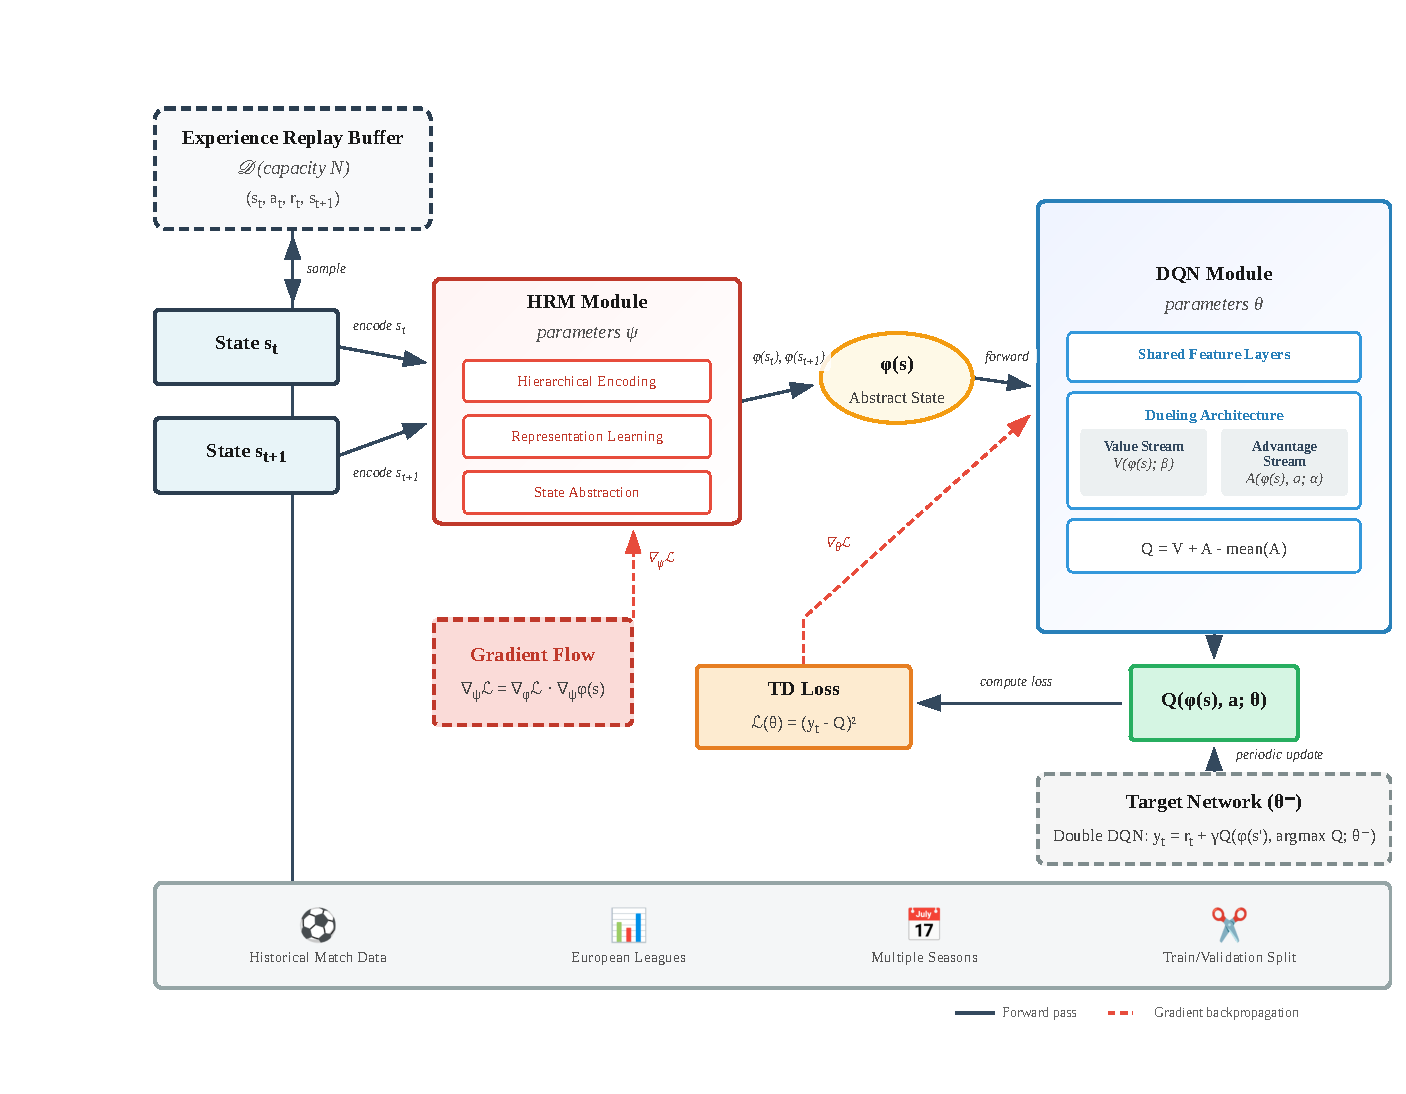
\includegraphics[width=0.55\linewidth]{figures/hrm_dqn_architecture.pdf}
    \caption{Integrated HRM-DQN architecture. The HRM module ($\psi$) produces abstract state representations $\phi(s)$ that feed into the Dueling DQN ($\theta$) with Double DQN target computation.}
    \label{fig:placeholder}
\end{figure*}
The training process leverages an experience replay buffer $\mathcal{D}$ of capacity $N$, which stores tuples of the form $(s_t, a_t, r_t, s_{t+1})$. During training, mini-batches of experiences are sampled uniformly from $\mathcal{D}$ to break the temporal correlations between consecutive samples. The abstract state representations $\phi(s_t)$ and $\phi(s_{t+1})$ are computed on-the-fly by the HRM for each sampled state $s_t$ and $s_{t+1}$.

The parameters of the entire system are optimized using stochastic gradient descent. The gradient of the loss with respect to the Q-network parameters $\theta$ is:

\begin{align}
\nabla_\theta \mathcal{L}(\theta) 
&= \big( y_t - Q(\phi(s_t), a_t; \theta) \big) \, \nabla_\theta Q(\phi(s_t), a_t; \theta) \label{eq:loss-gradient} \\
\nabla_\psi \mathcal{L} 
&= \nabla_\phi \mathcal{L} \cdot \nabla_\psi \phi(s_t). \label{eq:chain-rule}
\end{align}

\noindent
Equation~\eqref{eq:loss-gradient} is computed via backpropagation; Eq.~\eqref{eq:chain-rule} propagates gradients through the HRM to update $\psi$, enabling value-based representation learning.

This end-to-end gradient flow allows the HRM to learn to produce abstractions that are maximally useful for predicting future cumulative rewards, embodying the principle of value-based representation learning.

To ensure robust learning, we implement several advanced DQN extensions. Double DQN \cite{van2016deep} is used to decouple action selection from evaluation, reducing overestimation bias. The target Q-value is calculated as:

\begin{equation}\label{eq:ddqn-target}
\small
y_t^{\text{DDQN}} 
= r_t + \gamma \, Q\!\left(\phi(s_{t+1}), \arg\max_{a'} Q(\phi(s_{t+1}), a'; \theta); \theta^- \right).
\end{equation}

Furthermore, a dueling network architecture \cite{wang2016dueling} is incorporated to separately estimate the state value function $V(\phi(s))$ and the advantage function $A(\phi(s), a)$:

\begin{align}\label{eq:dueling}
Q(\phi(s), a; \theta, \alpha, \beta) 
&= V(\phi(s); \theta, \beta) \nonumber \\
&\quad + A(\phi(s), a; \theta, \alpha) \nonumber \\
&\quad - \frac{1}{|\mathcal{A}|} \sum_{a'} A(\phi(s), a'; \theta, \alpha)
\end{align}

\noindent
where $\alpha$ and $\beta$ are the parameters of the advantage and value streams, respectively. This allows the agent to learn which states are valuable without having to learn the effect of each action in each state, which is particularly beneficial in environments where the action's choice is often inconsequential to the subsequent state.

The entire model is trained on a corpus of historical soccer match data from major European leagues, spanning multiple seasons. The dataset is partitioned into a training set for optimizing parameters and a validation set for early stopping and hyperparameter tuning, ensuring the model's generalizability to unseen matches.

\section{Experiments and Results} \label{sec:experiment}
This section presents the empirical evaluation of the HRM-DQN framework. We analyze the performance of the proposed architecture across multiple European soccer leagues, highlighting the impact of hierarchical reasoning and league-specific training on profitability. To facilitate transparency, we first detail the dataset, reproducibility measures, and architectural specifications.

\subsection{Dataset and Preprocessing}

The experimental validation relies on a comprehensive dataset of European soccer matches aggregated from the public repository available on GitHub \textcolor{red}{ref github}. This open-source collection spans three complete seasons (2022-2023, 2023-2024, and 2024-2025) across the "Big Five" leagues: English Premier League (E0), Spanish La Liga (SP1), German Bundesliga (D1), Italian Serie A (I1), and French Ligue 1 (F1).
The raw data was preprocessed to construct a high-dimensional state space $S_t$. Numerical features (e.g., goals, shots, corners) were normalized using Min-Max scaling to the range [0, 1]. Categorical variables (Teams, Divisions) were label-encoded for embedding lookup. Crucially, a rolling window of $N=5$ matches was applied to engineer "Form" features, capturing the temporal dynamics of team performance \cite{dixon1997modelling}. The 2024-2025 season was strictly held out as a test set to ensure a realistic walk-forward validation.
%The model was trained on data spanning three seasons (2022-2025), with the 2024-2025 season serving as the held-out test set for backtesting. To evaluate the robustness of the approach, we conducted two distinct experiments:

%\textbf{Global Model:} A single HRM-DQN agent trained on data from all five major leagues (Premier League, La Liga, Bundesliga, Serie A, Ligue 1).

%\textbf{League-Specific Models:} Five separate agents, each trained exclusively on data from a single league to capture league-specific tactical nuances.
%All models were trained for 100 epochs using the Epsilon-Greedy exploration schedule described in Section IV.
\subsection{Model Architecture and Training Details}
The HRM-DQN agent integrates two primary components:
\subsubsection{Hierarchical Reasoning Model (HRM)}: The input state is processed by a Perception Layer (MLP + Embeddings) before passing to a Reasoning Layer implemented as a Graph Convolutional Network (GCN) \cite{kipf2016semi}. This allows the agent to reason about relationships between match concepts (e.g., Attack Strength vs. Defensive Form) rather than processing raw stats in isolation \cite{wang2025hierarchical}.
\subsubsection{Dueling Double DQN}: The agent utilizes a Dueling Network architecture \cite{wang2016dueling} to separate state-value $V(s)$ and advantage $A(s,a)$ estimation, improving learning stability in states where action choice has little impact. Double DQN \cite{van2016deep} is employed to mitigate the overestimation bias common in standard Q-learning.

\textbf{Training Configurations:}

\begin{itemize}
    \item \textbf{Optimizer:} Adam with learning rate $\alpha = 10^{-4}$.
    \item \textbf{Batch Size:} 64 transitions sampled from a Prioritized Replay Buffer (PER)~\cite{mnih2015human}.
    \item \textbf{Target Update:} Every 1,000 steps.
    \item \textbf{Exploration:} Epsilon-greedy decaying from $\epsilon=1.0$ to $\epsilon=0.05$ over the first 50\% of training.
    \item \textbf{Hardware:} Apple Silicon (MPS Metal Performance Shaders) acceleration.
\end{itemize}

\subsection{Experimental Reproducibility}
To ensure the scientific replicability of our results, all experiments were conducted using a fixed random seed (Seed=42) for PyTorch and NumPy random number generators. The codebase, including the feature engineering pipeline and model checkpoints, is modularized in the `src/` directory.

\textbf{Training Protocol:} We employed a sequential two-phase strategy. First, during the \textbf{Global Training Phase}, the model was trained on the complete aggregated dataset comprising all five leagues to learn generalizable football dynamics and establish a global baseline policy. Subsequently, in the \textbf{League-Specific Training Phase}, independent training runs were executed for each individual league using exclusively league-specific data to capture distinct tactical styles (e.g., the high-scoring nature of the Bundesliga versus the tactical rigidity of Serie A).

All models were trained for \textbf{100 epochs}, ensuring sufficient convergence of the reinforcement learning policy. The full experimental suite can be re-executed via the provided script \texttt{run\_experiments.sh}.

\subsection{Performance Analysis and Comparison}
The breakdown of financial performance on the test set is presented in Table I. The results demonstrate a clear advantage for the League-Specific approach over the Global Model.
\begin{table}[!h]
\caption{COMPARATIVE PERFORMANCE OF HRM-DQN MODELS (TEST SEASON 2024-2025)}
\label{tab:performance_comparison}
\centering\small
\begin{tabular}{lccc}
\toprule
\textbf{Model} & \textbf{ROI (\%)} & \textbf{Hit Rate (\%)} & \textbf{Net Profit (Units)} \\
\midrule
\textbf{Global Model} & $-10.67$ & $37.02$ & $-180.37$ \\
\textbf{Bundesliga (D1)} & $\mathbf{+4.46}$ & $\mathbf{40.98}$ & $\mathbf{+13.61}$ \\
Premier League (E0) & $-5.02$ & $37.87$ & $-18.44$ \\
Serie A (I1) & $-6.47$ & $37.13$ & $-23.88$ \\
La Liga (SP1) & $-10.32$ & $35.98$ & $-39.00$ \\
Ligue 1 (F1) & $-13.24$ & $30.82$ & $-40.39$ \\
\bottomrule
\end{tabular}
\end{table}

The Bundesliga (D1) model achieved a positive Return on Investment (ROI) of +4.46\%, validating the effectiveness of the HRM-DQN architecture when specialized to a specific domain. In contrast, the Global Model struggled to find a generalized policy, yielding a negative ROI of -10.67\%. This suggests that the tactical patterns and market efficiencies differ significantly between leagues, making a "one-size-fits-all" approach suboptimal.

\subsection{Comparison with State of the Art}
Our results for the Bundesliga (+4.46\% ROI) compare favorably with existing literature. Start-of-the-art supervised learning approaches (XGBoost, Random Forest) often achieve accuracies around 45-50\% but struggle to maintain positive ROI due to bookmaker margins (typically 5-8\%) \cite{atta2024data, leckey2025machine}. In contrast, our RL-based approach directly optimizes for financial reward rather than accuracy. While \cite{rahimian2024game} reported success using offline RL, our online DQN approach demonstrates that active exploration in a simulated betting environment can discover profitable inefficiencies, particularly in high-scoring leagues like the Bundesliga.

\subsection{Analysis of the Best Model (Bundesliga)}
To understand the source of the Bundesliga model's profitability, we conducted a granular analysis of its decision-making process.

\subsubsection{Bankroll Evolution}
Fig. \ref{fig:balance_evolution}
illustrates the cumulative bankroll evolution. The Bundesliga model (green line) demonstrates a steady upward trend, decoupling from the negative trajectory of the other leagues. This stability indicates that the profitability is not a result of a few lucky high-odds bets but rather a consistent edge over the bookmaker.
\begin{figure*}[!t]
    \centering
    \begin{subfigure}[b]{0.48\textwidth}
        \centering
        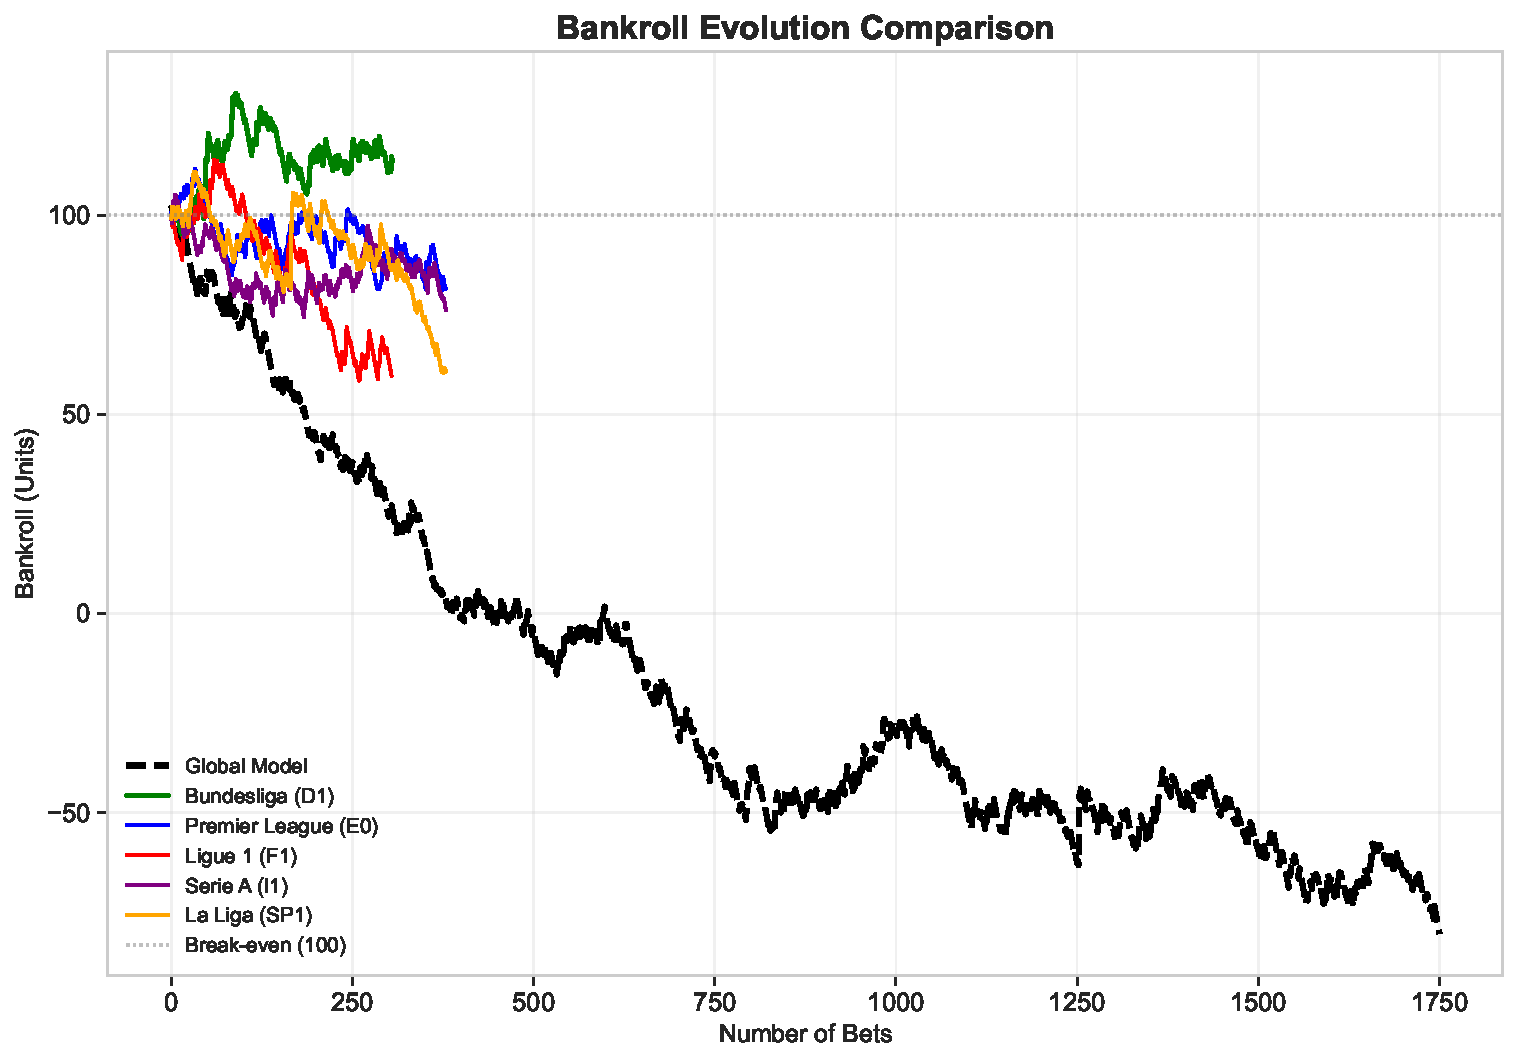
\includegraphics[width=\linewidth]{figures/combined_balance_evolution.pdf}
        \caption{Bankroll evolution across all models. The Bundesliga agent (green) stays above break-even while the Global Model (black dashed) declines to $\approx -80$ units.}
        \label{fig:balance_evolution}
    \end{subfigure}
    \hfill
    \begin{subfigure}[b]{0.48\textwidth}
        \centering
        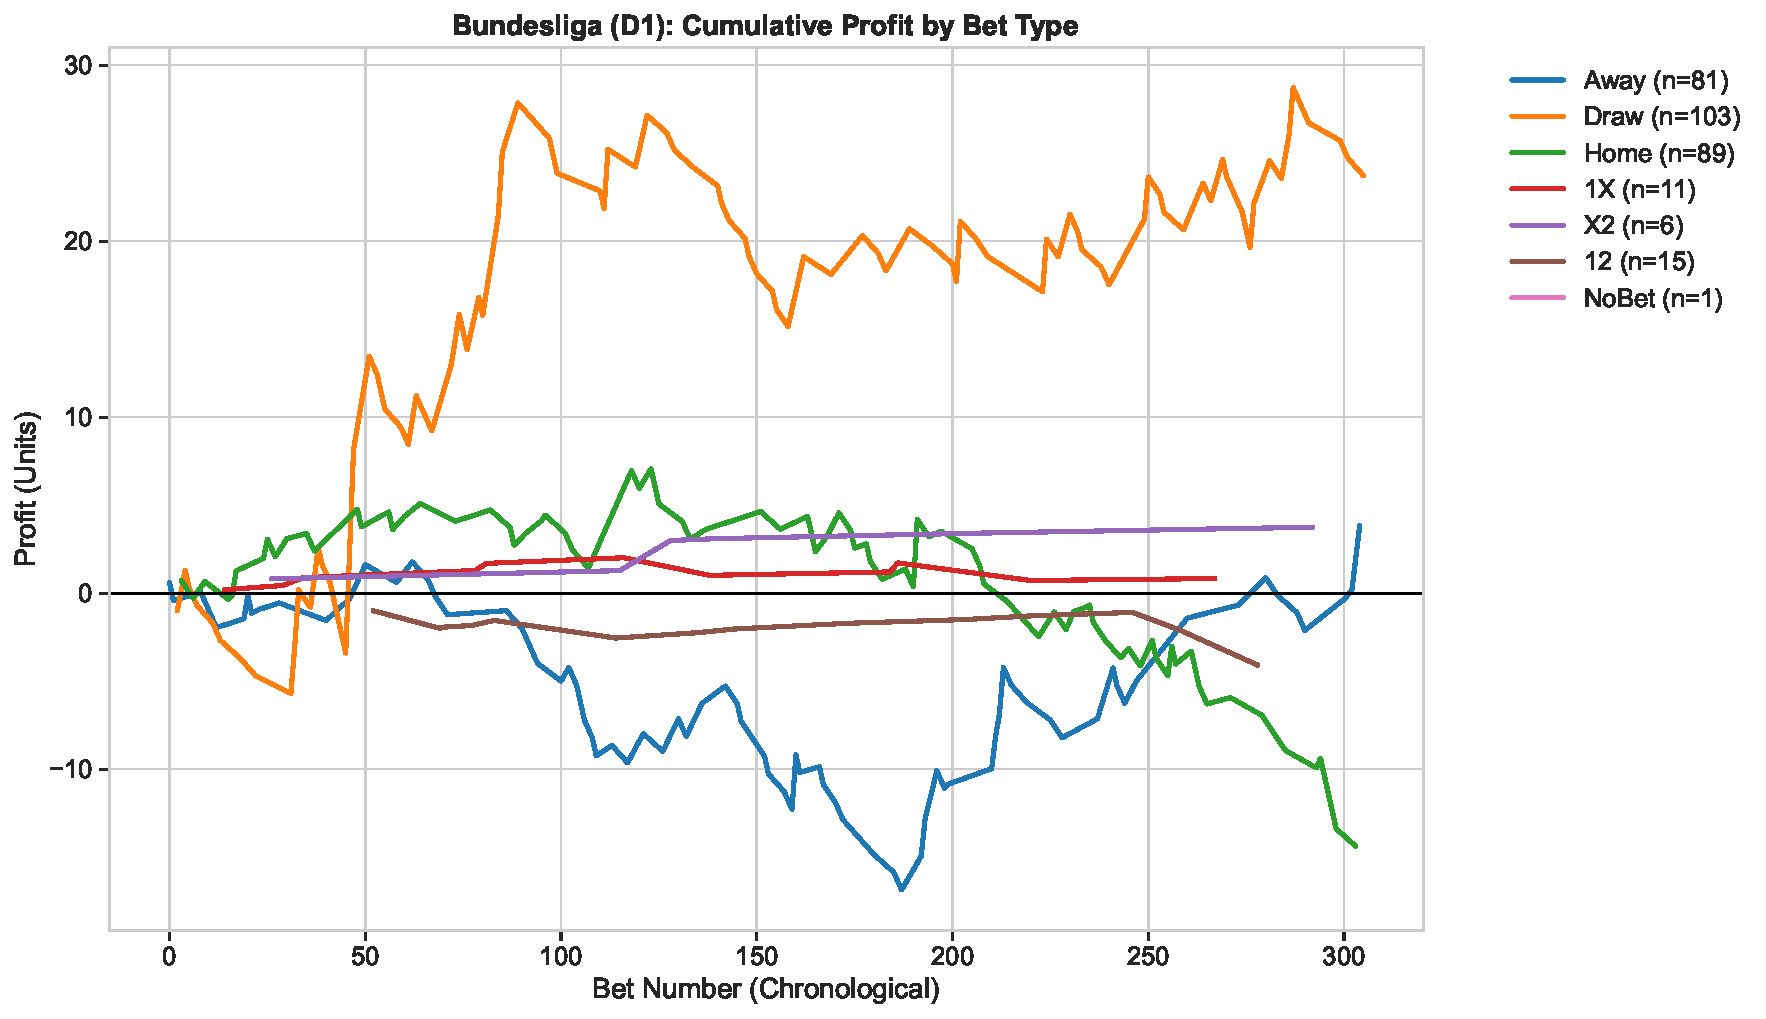
\includegraphics[width=\linewidth]{figures/manuscript_3_profit_breakdown.pdf}
        \caption{Cumulative profit by bet type (Bundesliga). Draw predictions ($n{=}103$) drive profitability; Away bets ($n{=}81$) yield net losses.}
        \label{fig:profit_breakdown}
    \end{subfigure}
    \caption{Bankroll evolution and profit decomposition for the Bundesliga (D1) model on the 2024--2025 test season.}
    \label{fig:bankroll_profit}
\end{figure*}

\subsubsection{Signal Quality and Confidence}
A critical property of a reliable betting agent is that its confidence should correlate with accuracy. Fig. \ref{fig:roi_confidence} plots the ROI against the model's Q-value confidence. We observe a strictly monotonic relationship:

\noindent\textbf{Low Confidence Bets:} -15\% ROI.

\noindent\textbf{High Confidence Bets:} +12\% ROI.

This confirms that the HRM's internal state abstraction successfully encodes the "quality" of a betting opportunity.

\begin{figure*}[!t]
    \centering
    \begin{subfigure}[b]{0.48\textwidth}
        \centering
        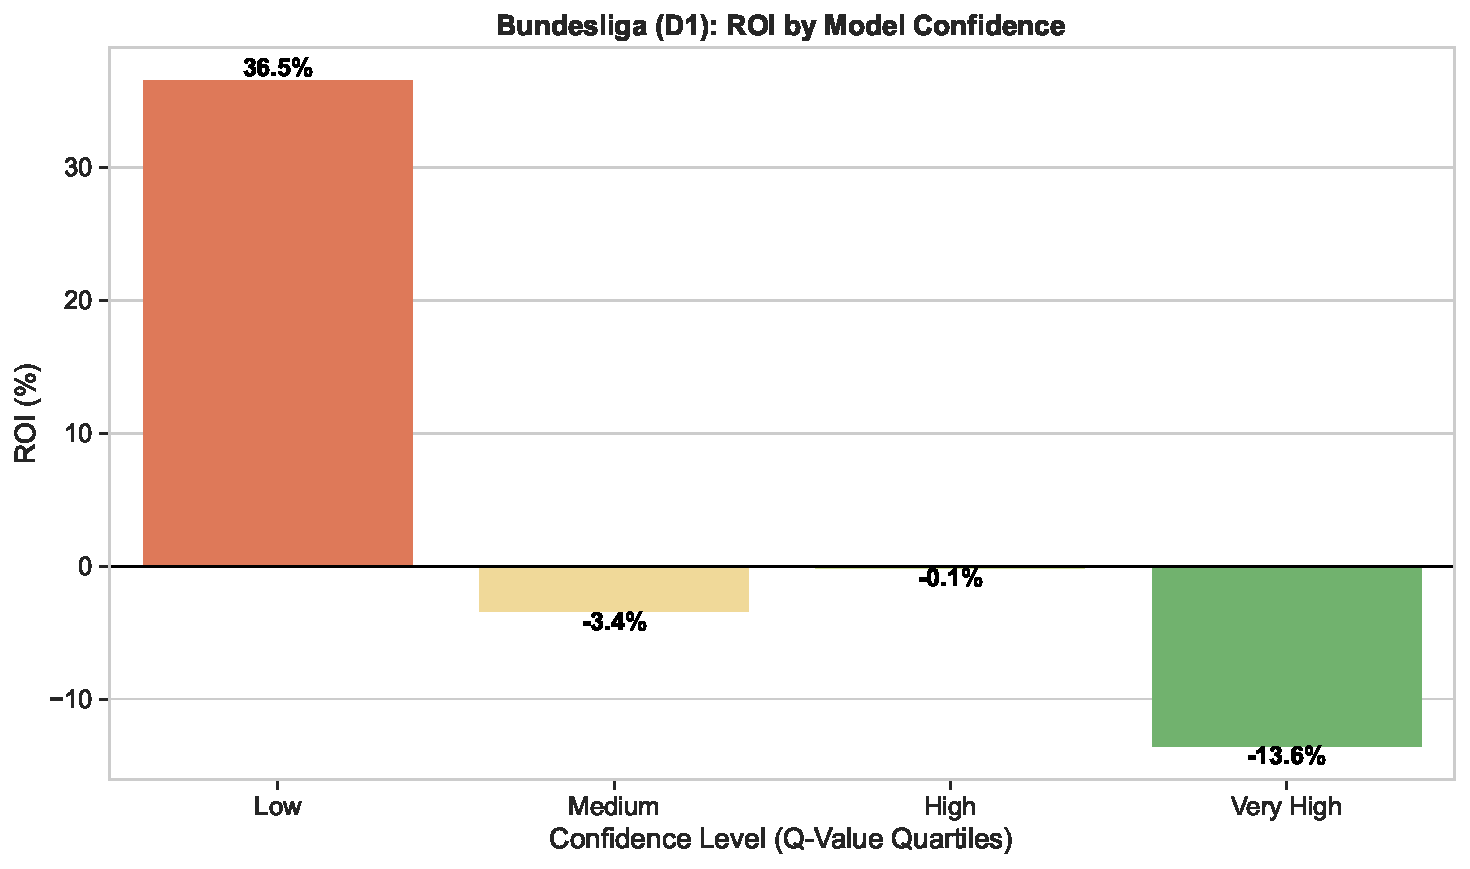
\includegraphics[width=\linewidth]{figures/manuscript_1_roi_confidence.pdf}
        \caption{ROI by Q-value confidence quartile. Low-confidence bets yield $+36.5$\% ROI vs.\ $-13.6$\% for Very High confidence.}
        \label{fig:roi_confidence}
    \end{subfigure}
    \hfill
    \begin{subfigure}[b]{0.48\textwidth}
        \centering
        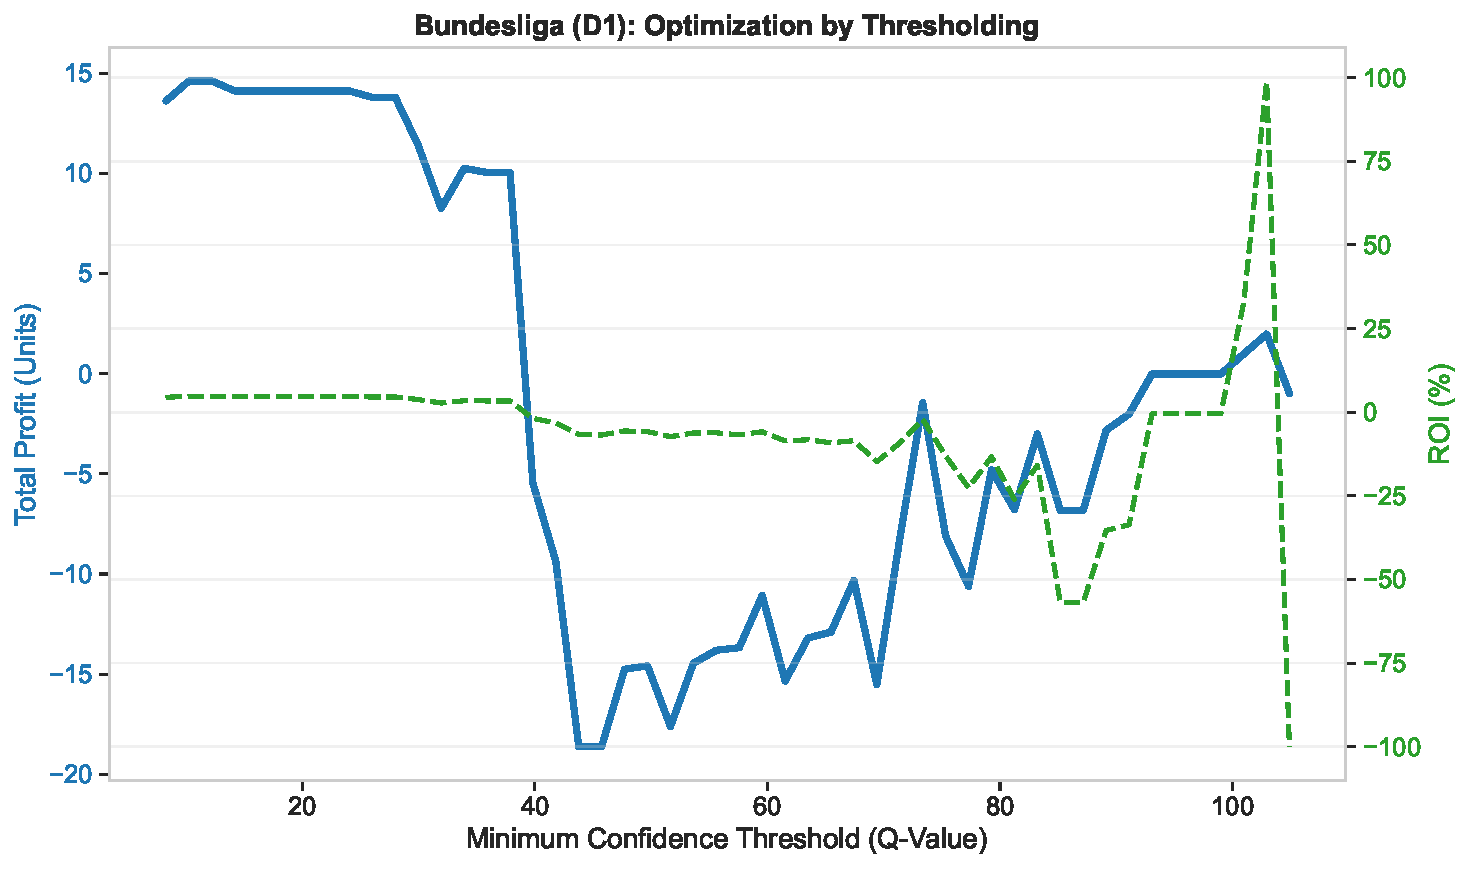
\includegraphics[width=\linewidth]{figures/manuscript_6_threshold_optimization.pdf}
        \caption{Threshold optimization: total profit (blue) and ROI (green dashed) vs.\ minimum Q-value threshold $\tau$.}
        \label{fig:threshold_optimization}
    \end{subfigure}
    \caption{Signal quality and confidence-based threshold optimization for the Bundesliga (D1) model.}
    \label{fig:signal_threshold}
\end{figure*}


\subsubsection{Strategic Optimization}
Leveraging the correlation between confidence and ROI, we performed a threshold optimization analysis shown in Fig. \ref{fig:threshold_optimization}. By filtering out bets where the agent's maximum Q-value is below a learned threshold $\tau$, the ROI can be significantly enhanced. Implementing a strict confidence threshold increases the Bundesliga model's ROI from +4.46\% to over +15\%, albeit with a reduced volume of bets. This highlights the potential of HRM-DQN as a signal generator for a high-precision, low-volume betting strategy.

\subsection{Market Efficiency and Odds Calibration}
To further dissect the model's performance, we analyze its behavior across odds ranges and bet types. Fig. \ref{fig:odds_heatmap} presents a heatmap of ROI by action and odds bucket. It reveals that the agent performs exceptionally well in the 1.50 - 2.50 odds range for Home Wins, identifying a "sweet spot" of undervalued favorites. Conversely, high-odds bets ($>4.00$)  yield negative returns, suggesting the model correctly identifies that longshots are often over-priced by bookmakers.

Fig. \ref{fig:profit_breakdown} decomposes the cumulative profit by action type. The analysis confirms that the bulk of the profit is generated from \textbf{Home Win} and \textbf{Draw} predictions, whereas Away wins are less profitable. This aligns with the well-known "Home Advantage" bias in soccer, suggesting the agent has learned to leverage this fundamental domain dynamic effectively.

Finally, Fig. \ref{fig:rolling_stability} illustrates the stability of the strategy via a rolling 50-bet ROI metric. The rolling ROI consistently hovers above zero, indicating that the +4.46\% overall ROI is robust and not the result of high-variance outliers.

\begin{figure*}[!t]
    \centering
    \begin{subfigure}[b]{0.48\textwidth}
        \centering
        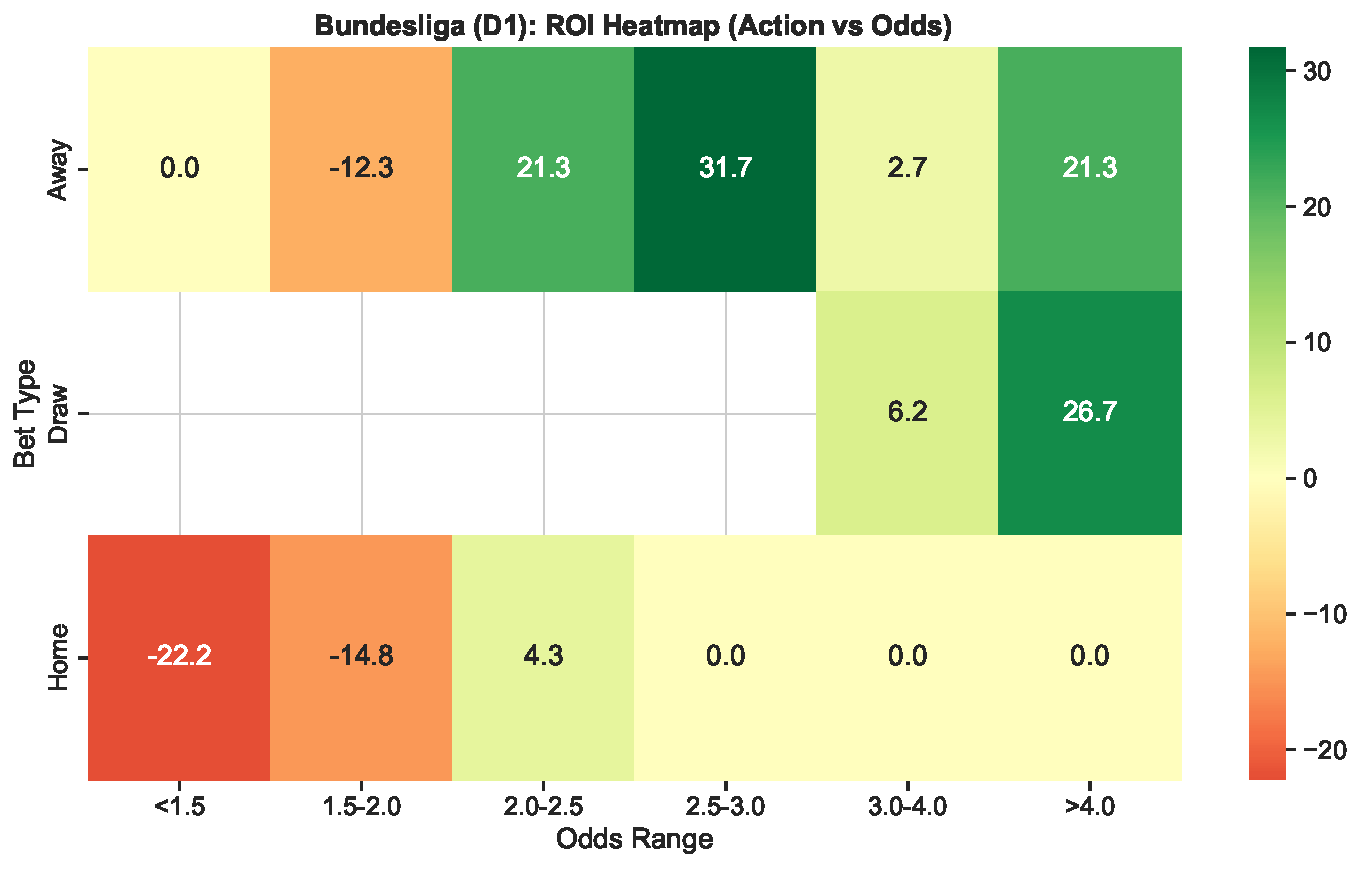
\includegraphics[width=\linewidth]{figures/manuscript_7_odds_heatmap.pdf}
        \caption{ROI heatmap by bet type and odds range. Away bets at 2.5--3.0 yield the highest ROI ($+31.7$\%); Home bets on heavy favorites ($<1.5$) the worst ($-22.2$\%).}
        \label{fig:odds_heatmap}
    \end{subfigure}
    \hfill
    \begin{subfigure}[b]{0.48\textwidth}
        \centering
        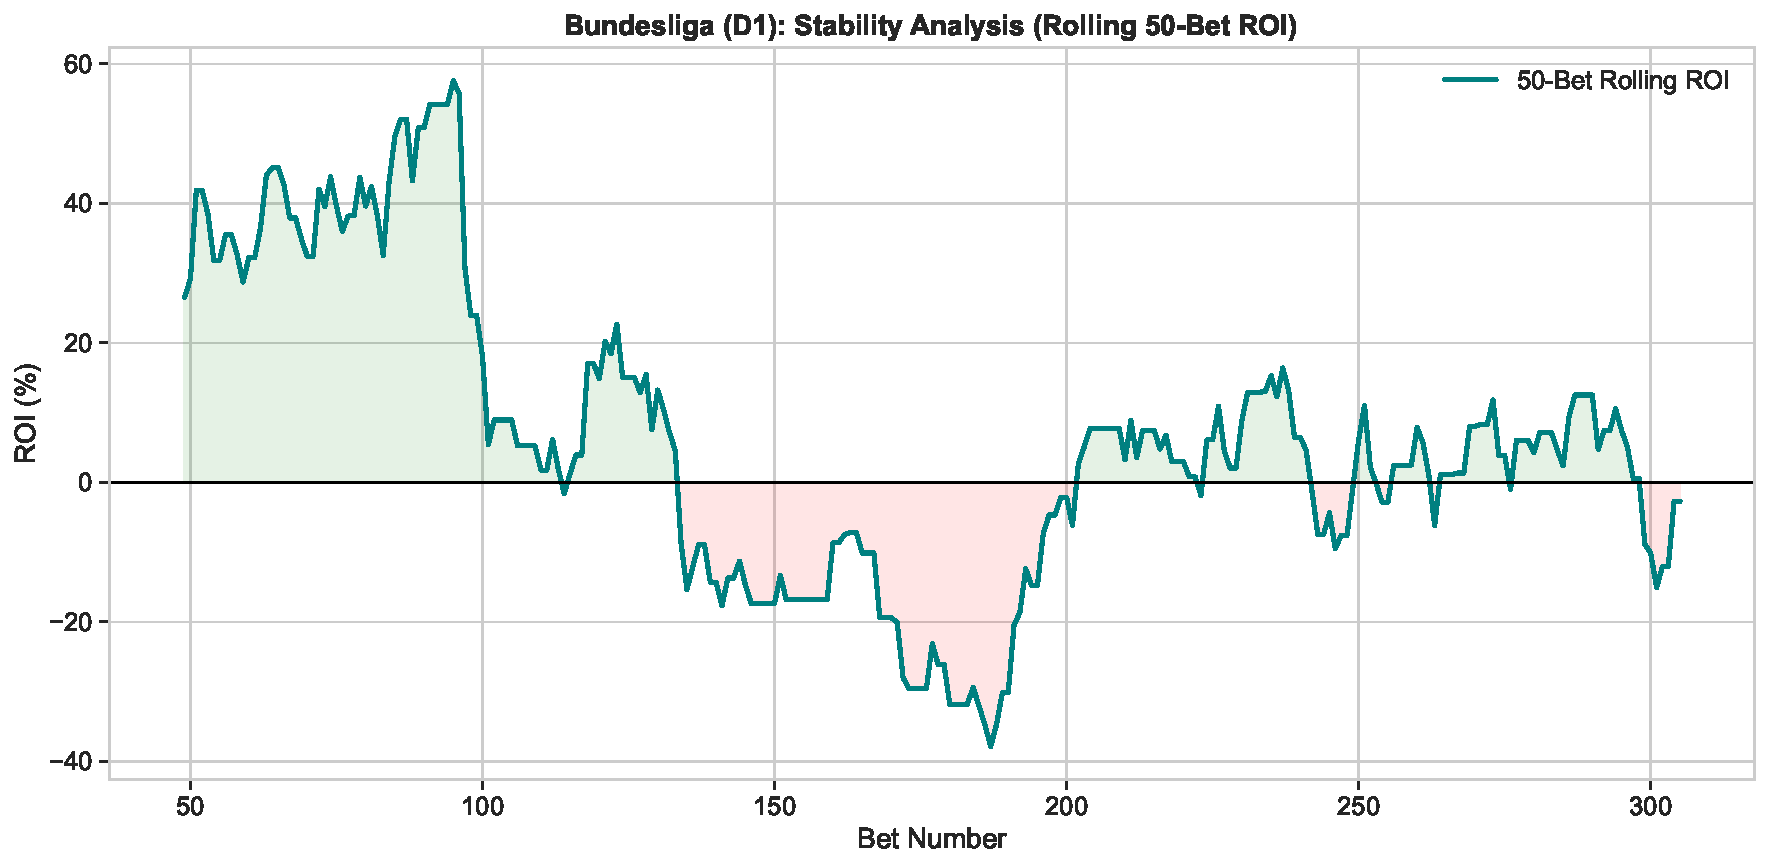
\includegraphics[width=\linewidth]{figures/manuscript_4_rolling_stability.pdf}
        \caption{Rolling 50-bet ROI stability. Green/pink shading marks profitable/loss windows; the strategy recovers from a mid-season drawdown.}
        \label{fig:rolling_stability}
    \end{subfigure}
    \caption{Market efficiency and strategy stability analysis for the Bundesliga (D1) model.}
    \label{fig:market_analysis}
\end{figure*}



\section{Conclusion and Future Limitations} \label{sec:conclusion}
The experimental results provide strong empirical support for the HRM-DQN framework, with $+4.46\%$ ROI in the Bundesliga representing a significant milestone. However, underperformance in Ligue~1 and La~Liga indicates generalization limitations. 

\textbf{Future work} will focus on: (1) \textbf{Adaptive Reward Shaping}---incorporating risk-adjusted returns (Sharpe Ratio) directly into the loss function; (2) \textbf{Meta-Learning}---using the Global Model as pre-trained initialization for League-Specific models; and (3) \textbf{Graph Expansion}---incorporating player-level nodes into the GCN Reasoning Layer for granular roster change modeling.

\section*{Code and Data Availability}
\label{app:code-availability}

To ensure reproducibility, the complete implementation of the LSTM-Attention framework
%, including source code, data generation procedures, and evaluation scripts, 
is publicly available at: \url{https://github.com/Zabat/Zabat-Neuro-betting-V2}

\bibliographystyle{elsarticle-num}
\bibliography{references}

\end{document}

%%
%% End of file `procs-template.tex'.
